\documentclass{article}
\usepackage{graphicx}
\usepackage{amsmath}
\usepackage{hyperref}
\usepackage{geometry}
\usepackage{booktabs}
\usepackage{ctex}

\geometry{a4paper, margin=1in}

\title{模型训练报告}
\author{王宝德}
\date{\today}

\begin{document}
	
\maketitle

\tableofcontents
\newpage

\section{项目背景}

\subsection{数据概述}
训练集42346条样本,共分为9类;验证集4229条样本,一共8类; 测试集4238条样本,一共8类。
	
\begin{table}[h!]
	\centering
	\begin{minipage}[b]{0.25\textwidth}
		\centering
		\caption{训练集标签统计}
		\begin{tabular}{|l|r|}
			\hline
			\textbf{意图} & \textbf{计数} \\
			\hline
			餐馆 & 12335 \\
			景点 & 11930 \\
			酒店 & 11132 \\
			thank & 5320 \\
			出租 & 745 \\
			地铁 & 698 \\
			没有意图 & 169 \\
			bye & 14 \\
			greet & 3 \\
			\hline
		\end{tabular}
		
	\end{minipage}
	\hspace{0.05\textwidth} % 调整表格之间的间距
	\begin{minipage}[b]{0.3\textwidth}
		\centering
		\caption{验证集标签统计}
		    \begin{tabular}{|l|r|}
			\hline
			\textbf{意图} & \textbf{计数} \\
			\hline
			餐馆 & 1214 \\
			景点 & 1195 \\
			酒店 & 1114 \\
			thank & 540 \\
			出租 & 81 \\
			地铁 & 68 \\
			没有意图 & 16 \\
			bye & 1 \\
			\hline
		\end{tabular}

	\end{minipage}
	\hspace{0.05\textwidth} % 调整表格之间的间距
	\begin{minipage}[b]{0.25\textwidth}
    	\centering
		\caption{测试集标签统计}
	    \begin{tabular}{|l|r|}
			\hline
			\textbf{意图} & \textbf{计数} \\
			\hline
			餐馆 & 1268 \\
			景点 & 1171 \\
			酒店 & 1086 \\
			thank & 529 \\
			地铁 & 84 \\
			出租 & 76 \\
			没有意图 & 23 \\
			bye & 1 \\
			\hline
		\end{tabular}
	\end{minipage}
	
\end{table}

	根据上面三个表格可以看出样本分布不平衡,特别是bye和greet数量很少,如无特殊要求,可以不处理或者删掉,模型对其识别能力较差。除此以外,出租,地铁,没有意图数量相对较少,可以先根据模型的表现决定是否进行过采样训练增强对其的识别能力。

	训练集语料字符数平均为26.58,最长为97,最短为1;查看语料较短的情况,有两个样本为?,标签为出租,没有意图;一个为?,标签为酒店,我删除了这三个样本,避免影响模型训练。其他较短的语料未发现不合理标签。
	
	\section{模型选择与设计}
	
	因为训练集整体不大,因此模型不能设计的过大,按照给定的模型结构,并在最后增加分类层。
		
	\subsection{初始超参数设置}
	\begin{itemize}
		\item \textbf{学习率}:0.001
		\item \textbf{批量大小}: 32
		\item \textbf{训练轮数}: 100
		\item \textbf{优化器}: Adam
	\end{itemize}
	
	\section{实验结果与分析}
	
	\subsection{模型性能}
	保存训练过程中在验证集上表现最好的模型,使用测试集验证效果:
	
	\begin{table}[h]
		\centering
		\caption{模型性能评估}
		\begin{tabular}{lccc}
			\toprule
			\textbf{指标} & \textbf{训练集} & \textbf{验证集} & \textbf{测试集} \\
			\midrule
			F1-macro & 0.8699 & 0.9005 & 0.9225 \\
			F1-micro & 0.9882 & 0.9446 & 0.9441 \\
			\bottomrule
		\end{tabular}
	\end{table}
	
	因为数据集是不均衡的,宏平均效果要略差于微平均,表明对数量较少的类别识别效果略差。
	
	\subsection{损失函数曲线}

	\begin{figure}[htbp]
		\centering
		\begin{minipage}[b]{0.3\textwidth}  
			\centering
			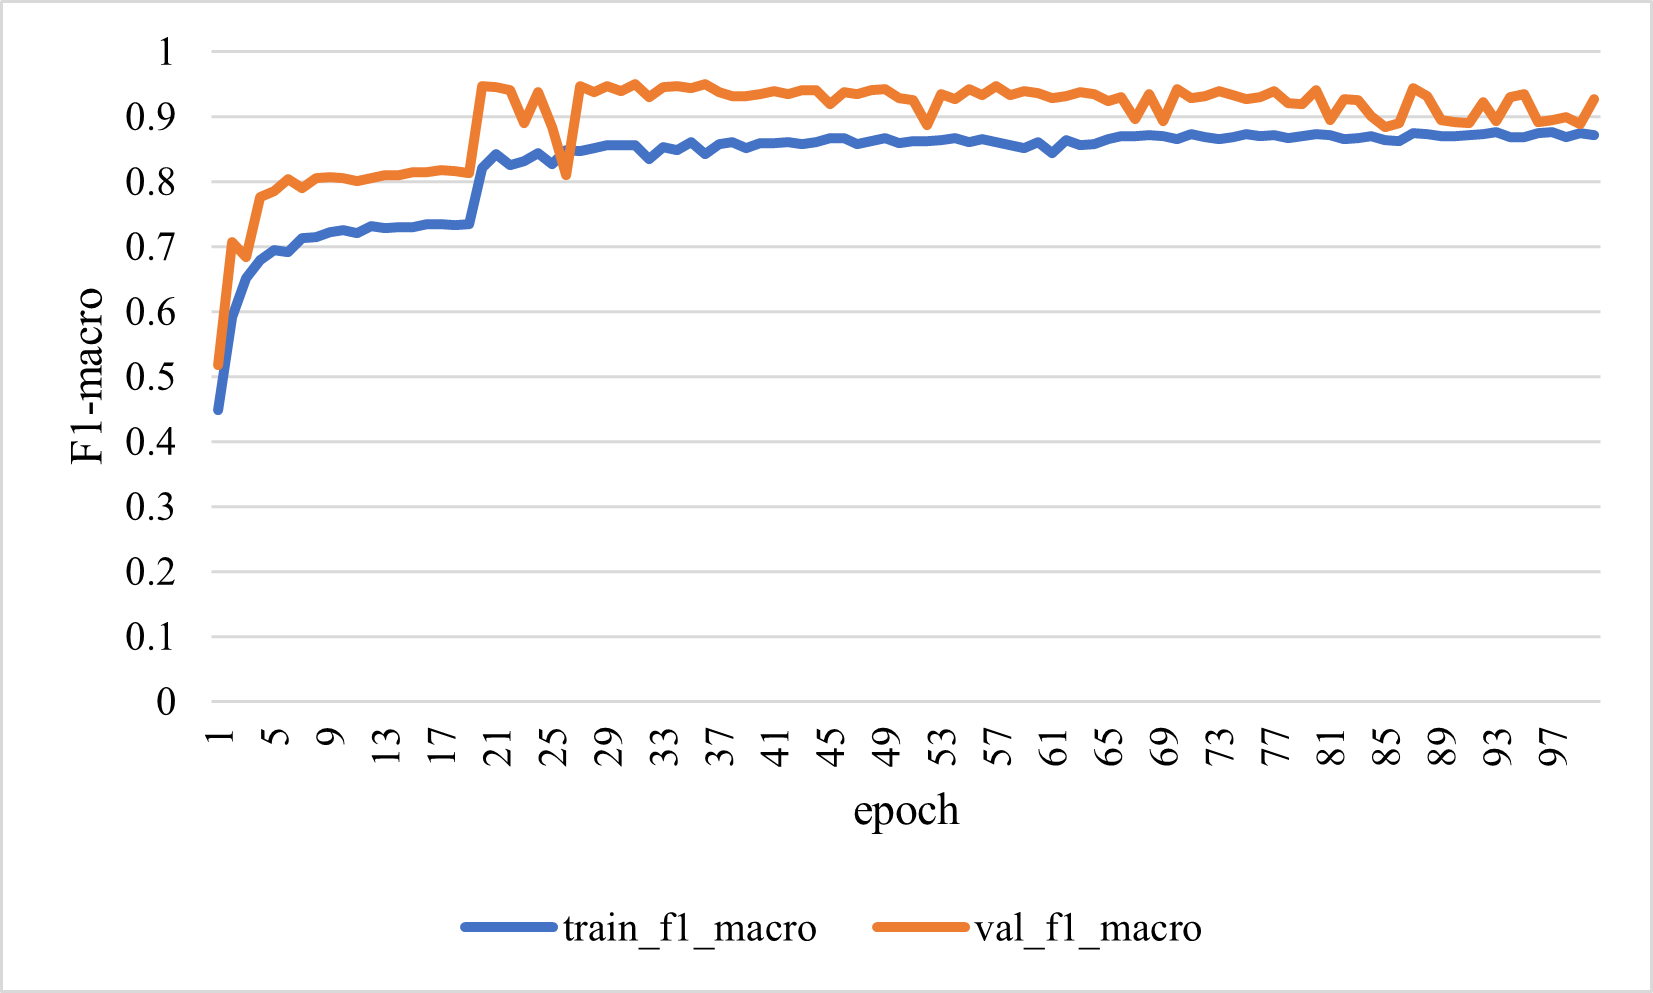
\includegraphics[width=\textwidth]{f1macro.png}
			\caption{训练集和测试集F1-macro随训练变化}
			\label{fig:f1macro}
		\end{minipage}
		\hspace{0.05\textwidth} 
		\begin{minipage}[b]{0.3\textwidth} 
			\centering
			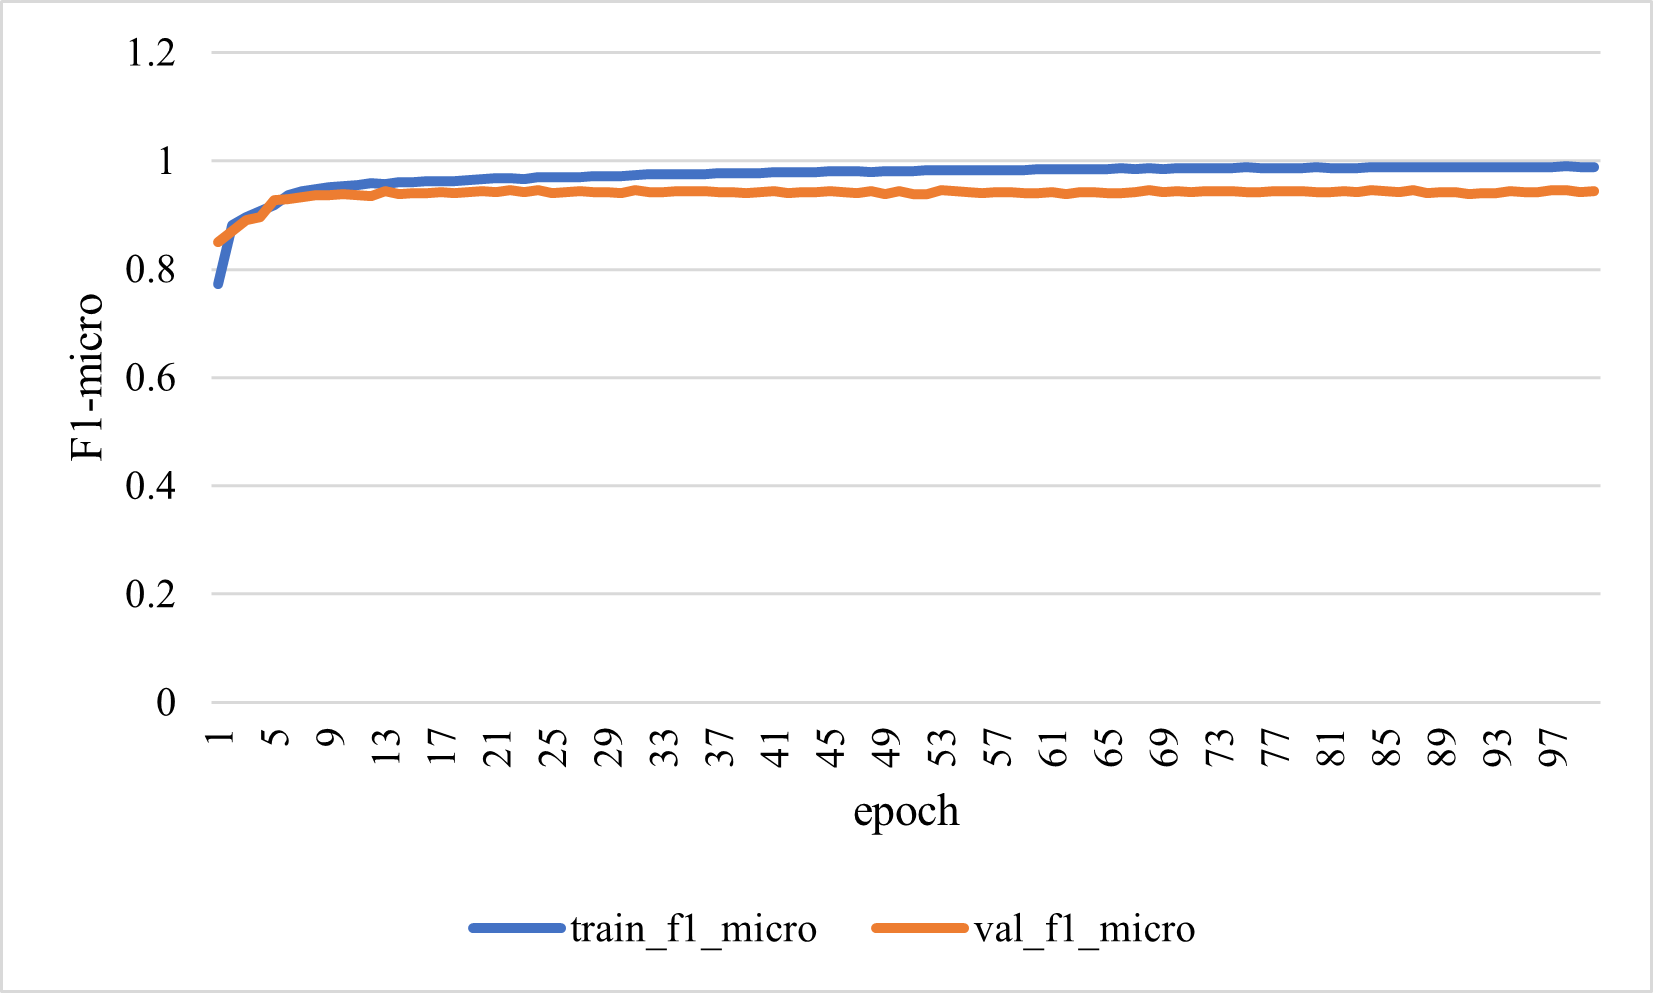
\includegraphics[width=\textwidth]{f1micro.png}
			\caption{训练集和测试集F1-micro随训练变化}
			\label{fig:f1micro}
		\end{minipage}
		\hspace{0.05\textwidth}  
		\begin{minipage}[b]{0.3\textwidth}  
			\centering
			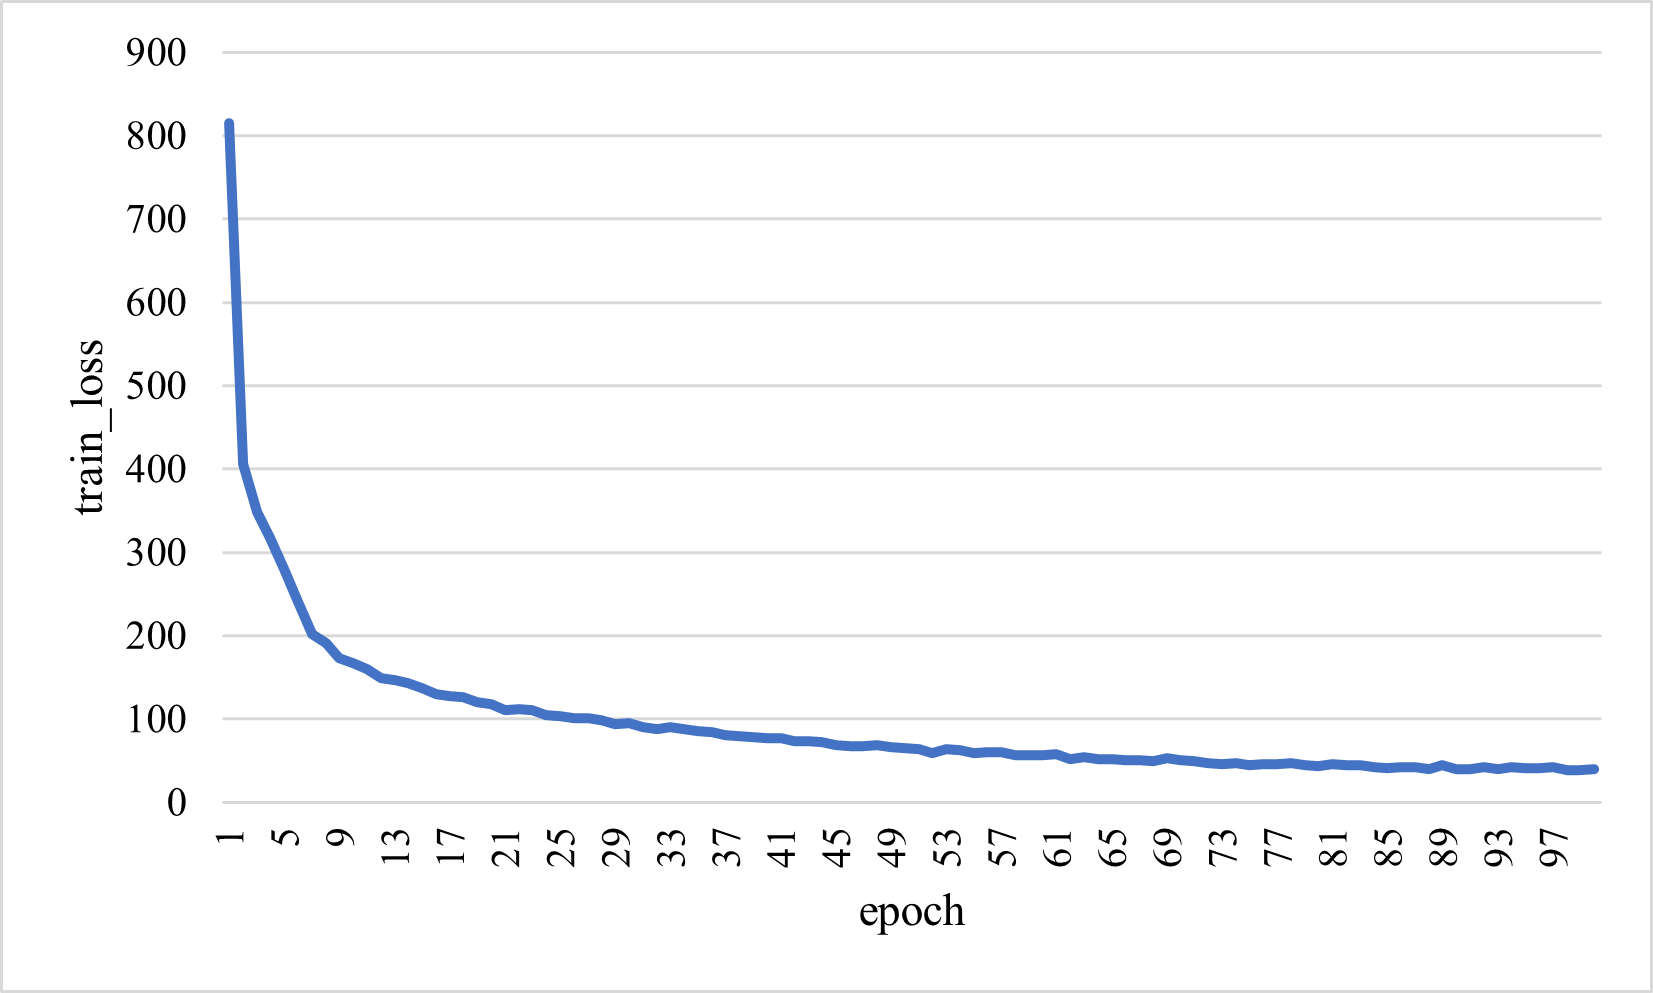
\includegraphics[width=\textwidth]{train_loss.png}
			\caption{训练损失变化}
			\label{fig:train_loss}
		\end{minipage}
	\end{figure}
	
	训练损失整体平稳下降,F1-micro变化也平稳,但是F1-macro曲线在训练过程中波动较大。但是有几个类的数量较少,在训练过程中对量少样本预测的轻微变化就会导致F1-macro发生较大变化,这也属正常情况,因此不处理。
	
	\subsection{模型优化与调优}
	初试是学习率设置为0.001,模型没有收敛,手动调到0.0001,验证集的F1-macro和F1-micro均达到了0.9以上,没有继续使用学习率调度器优化。
	
	
	\subsection{总结}
	总的来说,模型结构较为简单,容易收敛,在本数据集上,各种指标相对一致,模型分类效果较好。
	
	
\end{document}
